\section{其他技术说明}
\subsection{检查孔和检查孔盖}
检查传动零件的啮合情况,向箱体中注入润滑油。检查孔应设在上箱盖顶部能够直接观察到齿轮啮合部位的地方。检查孔为长方形,其大小应允许将手伸入箱内,以便检验齿轮啮合条件。检查孔盖用铸铁、钢板或有机玻璃制成,与箱体之间应加密封垫片。检查孔的盖板用螺钉固定在箱盖上。

检查孔和检查孔盖的主要尺寸设计如下:
\begin{figure}[h]
    \centering
    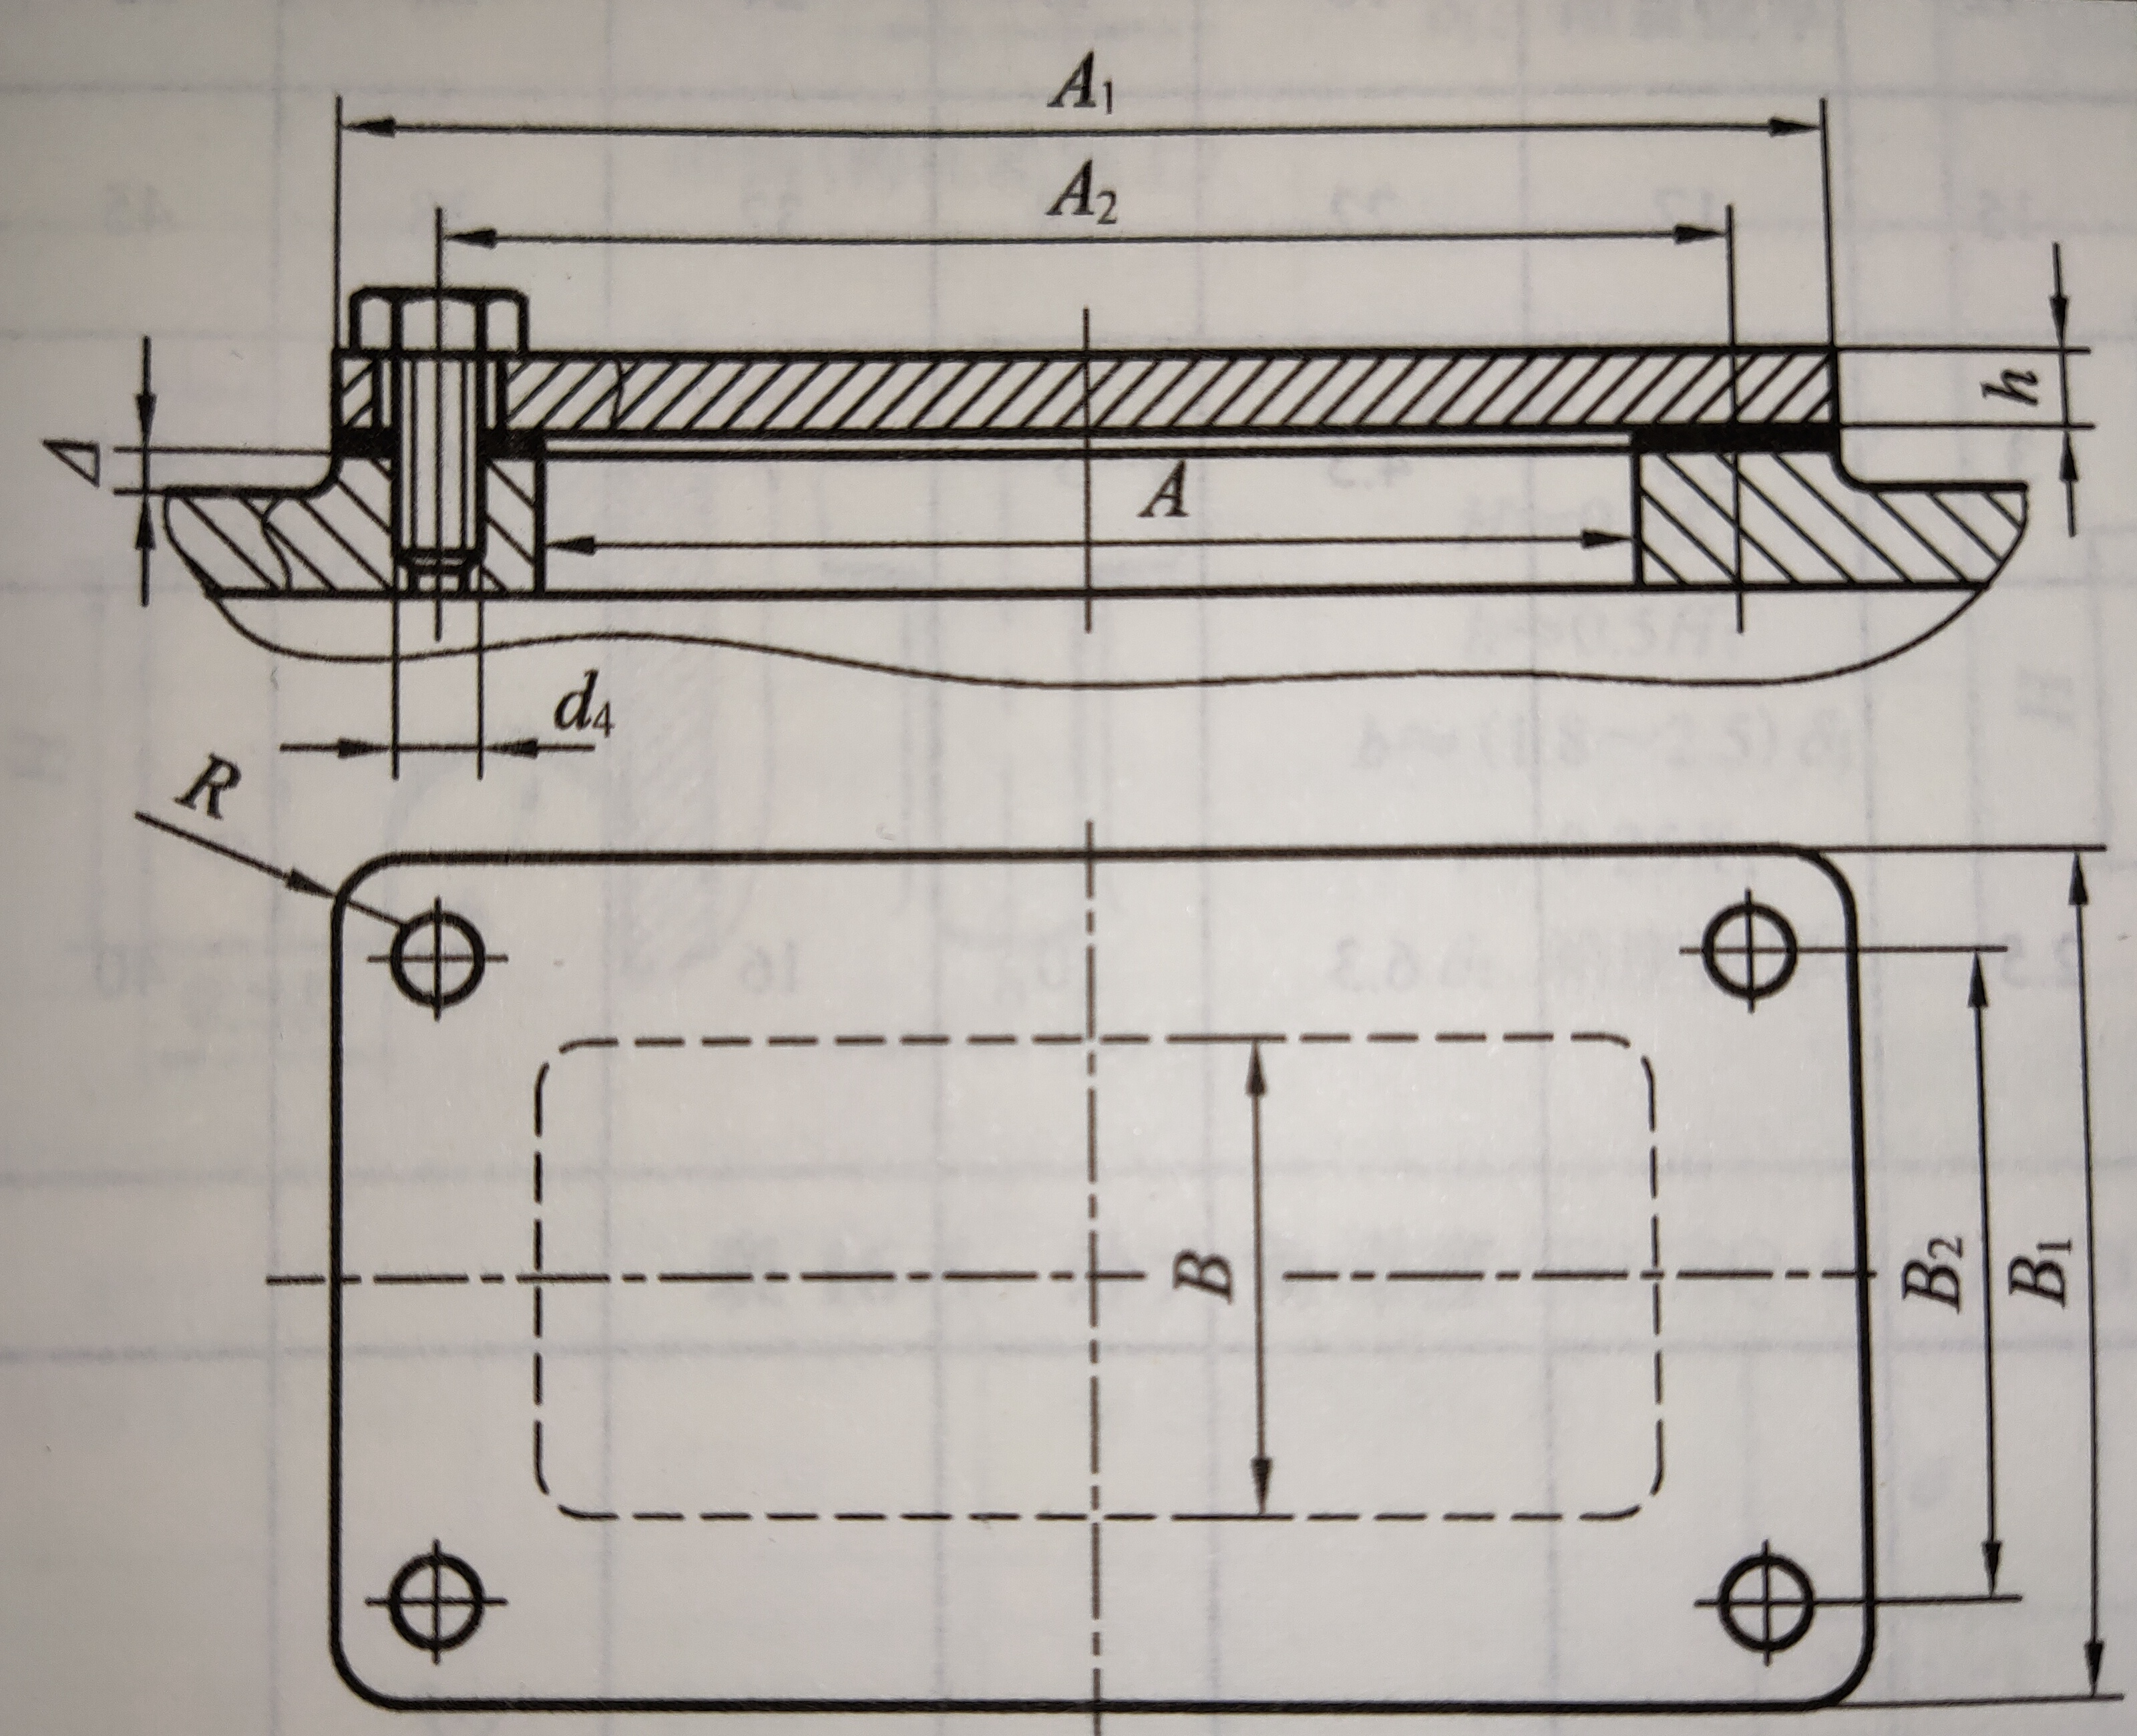
\includegraphics[scale=0.1]{graphic/10-1.jpg}
    \caption{轴的结构设计图检查孔和检查孔盖}
\end{figure}
查机械设计课程表$16-1$得具体尺寸如下:

$A=120mm,d_4=6mm,A1=A+5d_4=150mm,A_2=135mm,B_1=132mm$

$B=B_1-5d_4=102mm,B_2=117mm,R=6mm,H=3mm,\Delta=3mm$
\subsection{通气孔}
减速器工作,箱体内温度升高,气体膨胀,压力增大。通常在箱体顶部装设通气孔,使箱体内外压力平衡,不致使润滑油沿分箱面缝隙渗漏。垂直相通气孔的通气螺塞,其结构较为简单。若环境多尘可采用有滤网、防尘效果好的通气孔。

通气孔的主要尺寸设计如下:
\begin{figure}[h]
    \centering
    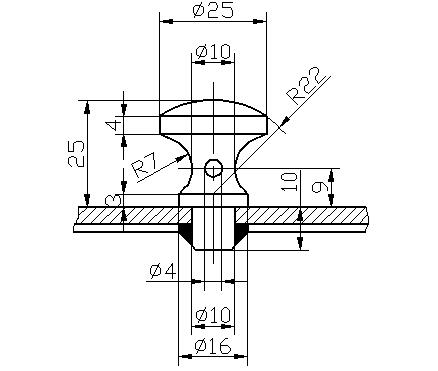
\includegraphics[scale=0.45]{graphic/10-2.jpg}
    \caption{通气孔}
\end{figure}
\subsection{定位销}
为了精确地加工轴承座孔,并保证每次拆装后轴承座的上下半孔始终保持制造加工时的位置精度,应在精加工轴承座前,在上箱盖和下箱盖的连接凸缘上配装定位销。采用的两定位圆锥销分别安置在箱体纵向和横向两侧的连接凸缘上,成非对称布置以加强定位效果。
\subsection{油面指示器}
用来指示箱体内油面的高度,油标位在便于观察减速器油面及油面稳定之处。油尺安置的部位不能太低,以防油进入油尺座孔二溢出。
\begin{figure}[h]
    \centering
    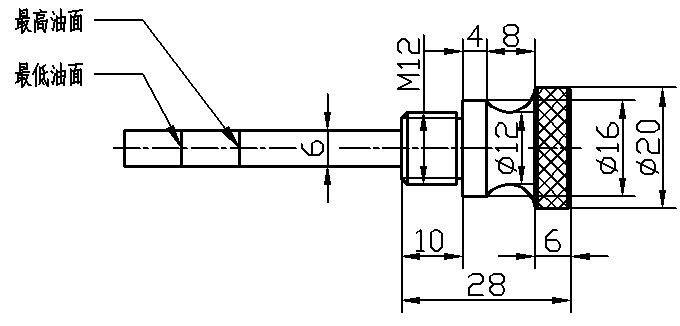
\includegraphics[scale=0.45]{graphic/10-5.jpg}
    \caption{油面指示器}
\end{figure}

\subsection{放油螺塞}
为排放减速器箱体内的污油和便于清洗箱体内部,在箱座油池的最低处设置放油孔,箱体内底面做成斜面,使油易于流出。
\begin{figure}[h]
    \centering
    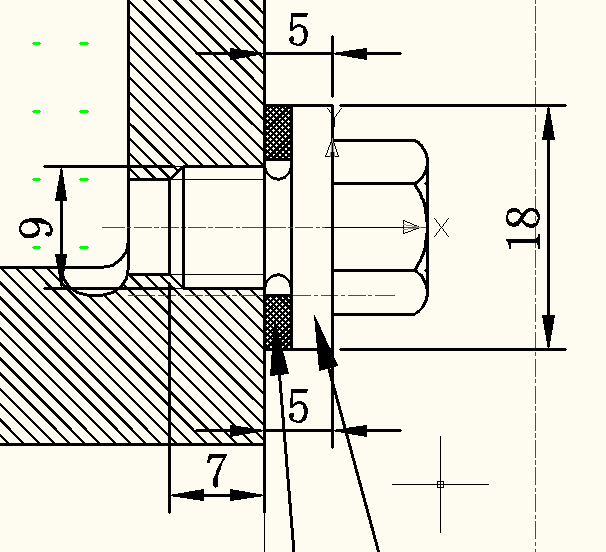
\includegraphics[scale=0.45]{graphic/10-6.png}
    \caption{放油螺塞}
\end{figure}

\subsection{起盖螺钉}
由于装配减速器时在箱体剖分面上涂有密封用的水玻璃或密封胶,因而在拆卸时往往因为胶结紧密难于开盖,旋动起盖螺钉可将箱盖顶起。选用的尺寸如图\ref{img4}

\begin{figure}[h]
    \centering
    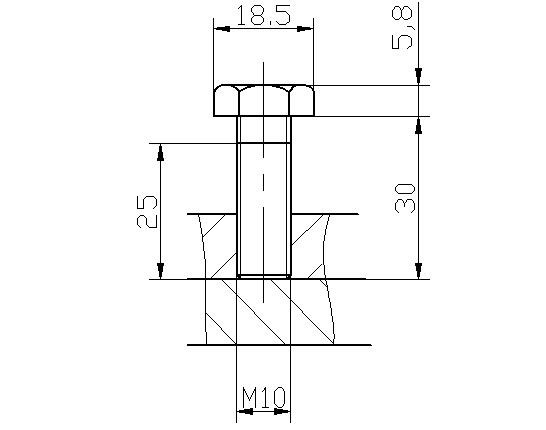
\includegraphics[scale=0.43]{graphic/10-4.jpg}
    \caption{起盖螺钉}
    \label{img4}
\end{figure}

\subsection{起吊装置}
起吊装置用于拆卸及搬运减速器。本设计采用吊环和吊耳。相关示例如\ref{img3}
\begin{figure}[h]
    \centering
    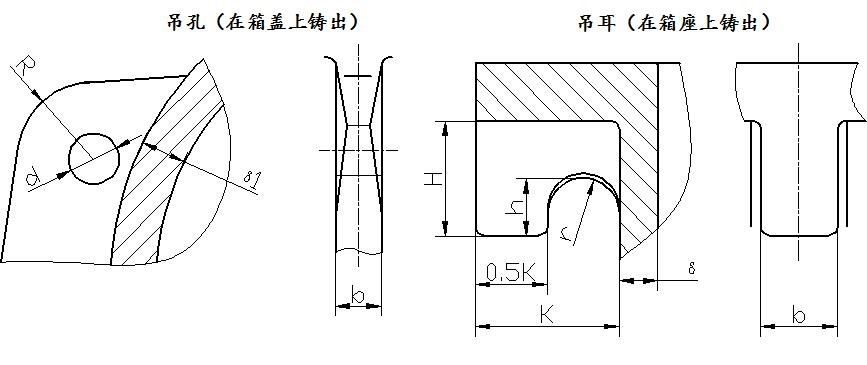
\includegraphics[scale=0.45]{graphic/10-3.jpg}
    \caption{起吊装置}
    \label{img3}
\end{figure}

吊孔尺寸计算
\[
b=2\delta_1=2\times 20=20mm
\]
\[
R= d=b=20mm
\]
\[
e=d=20mm
\]

吊耳尺寸计算

\[
K=C_1+C_2=20+16=36mm
\]
\[
H=0.8K=28.8mm
\]
\[
h=0.5H=14.4mm
\]
\[
r=0.25k=9mm
\]
